% RODAR PDF
% 1. ter o MikTex instalado
% 2.  pdflatex artigo.tex; bibtex artigo; pdflatex artigo.tex; pdflatex artigo.tex
% 3.  start artigo.pdf

% PDF SEMPRE ATUALIZADO
% 1. instale o strawberry perl
% 2. latexmk -pdf -pvc artigo.tex

%OU
% latexmk -C
% latexmk -pdf apresentacao.tex

\documentclass[aspectratio=169]{beamer}

% Pacotes essenciais
\usepackage[utf8]{inputenc}
\usepackage[T1]{fontenc}
\usepackage[brazilian]{babel}
\usepackage{graphicx}
\usepackage{tikz}

% Fonte moderna Roboto
\usepackage[sfdefault]{roboto}
\usepackage[T1]{fontenc}

% Definição das cores
\definecolor{vermelhoPrincipal}{HTML}{b11116}
\definecolor{azulComplementar}{HTML}{3a5461}
\definecolor{brancoFundo}{HTML}{FFFFFF}

% Configuração do tema
\usetheme{Madrid}
\usecolortheme{default}

% Cores personalizadas - texto sempre em preto
\setbeamercolor{structure}{fg=black}
\setbeamercolor{palette primary}{bg=vermelhoPrincipal,fg=white}
\setbeamercolor{palette secondary}{bg=azulComplementar,fg=white}
\setbeamercolor{palette tertiary}{bg=vermelhoPrincipal,fg=white}
\setbeamercolor{palette quaternary}{bg=azulComplementar,fg=white}
\setbeamercolor{frametitle}{bg=vermelhoPrincipal,fg=white}
\setbeamercolor{background canvas}{bg=brancoFundo}
\setbeamercolor{title}{fg=black}
\setbeamercolor{subtitle}{fg=azulComplementar}
\setbeamercolor{author}{fg=black}
\setbeamercolor{date}{fg=black}
\setbeamercolor{itemize item}{fg=black}
\setbeamercolor{itemize subitem}{fg=black}
\setbeamercolor{enumerate item}{fg=black}
\setbeamercolor{block title}{bg=vermelhoPrincipal,fg=white}
\setbeamercolor{block body}{bg=vermelhoPrincipal!10,fg=black}
\setbeamercolor{normal text}{fg=black}

% Configurar fonte dos itemize
\setbeamerfont{itemize/enumerate body}{size=\scriptsize}
\setbeamerfont{itemize/enumerate subbody}{size=\scriptsize}

% Marcadores modernos e minimalistas
\setbeamertemplate{itemize item}{\raisebox{0.2ex}{\rule{0.6ex}{0.6ex}}}
\setbeamertemplate{itemize subitem}{\raisebox{0.3ex}{\rule{0.4ex}{0.4ex}}}
\setbeamertemplate{itemize subsubitem}{\raisebox{0.35ex}{\rule{0.3ex}{0.3ex}}}
\setbeamertemplate{enumerate items}[square]

% Transições suaves
\setbeamercovered{transparent}

% Remover símbolos de navegação
\setbeamertemplate{navigation symbols}{}

% Customizar o cabeçalho com barra vermelha e logo
\setbeamertemplate{headline}{
  \begin{beamercolorbox}[wd=\paperwidth,ht=0.6cm,dp=0.15cm,leftskip=0.2cm,rightskip=0.4cm]{palette primary}
    \raisebox{-0.05cm}{
\includegraphics[height=0.45cm]{imgs/base/fatec-rgt.png}}
    \hfill
    \raisebox{-0.18cm}{
\includegraphics[height=0.85cm]{imgs/base/governo-sp-secretaria-logo.png}}
    \hspace{0.2cm}
    \raisebox{-0.08cm}{
\includegraphics[height=0.6cm]{imgs/base/cps-logo.png}}
  \end{beamercolorbox}
}
% Remover sombras dos blocks
\setbeamertemplate{blocks}[default]
\setbeamertemplate{itemize/enumerate body begin}{\scriptsize}
\setbeamertemplate{itemize/enumerate subbody begin}{\scriptsize}
% Customizar o rodapé
\setbeamertemplate{footline}{
  \begin{beamercolorbox}[wd=\paperwidth,ht=0.4cm,dp=0.2cm,leftskip=0.3cm,rightskip=0.3cm]{palette secondary}
    \usebeamerfont{footline}
    \insertshortauthor \hfill \hfill {\fontsize{5}{6}\selectfont\insertshorttitle} \hfill \hfill \insertframenumber/\inserttotalframenumber
  \end{beamercolorbox}
}

% Customizar título do frame
\setbeamertemplate{frametitle}{
  \vspace{0.3cm}
  \textcolor{black}{\insertframetitle}
  \vspace{0.1cm}
}

% Informações da apresentação
\title{Sistema para Auxílio de Revisão Sistemática, Orientado por PLN}
\subtitle{}
\author[DSM]{EGEN, B.; LINO, G.; DUTRA, P.; KOYAMA, Y.; SANTOS, S.}
\institute{Desenvolvimento de Software Multiplataforma\\FATEC Registro}
\date{\today}

\begin{document}

% Slide de título moderno
\begin{frame}
  \vspace{0.8cm}
  \begin{center}
    \begin{tikzpicture}
      % Linha decorativa superior
      \draw[vermelhoPrincipal, line width=2pt] (-4,0) -- (4,0);
    \end{tikzpicture}
    
    \vspace{0.4cm}
    
    {\normalsize\bfseries\inserttitle}\par
    
    \vspace{0.2cm}
    
    {\tiny\insertauthor}\par
    
    \vspace{0.1cm}
    
    {\small\textcolor{azulComplementar}{\insertsubtitle}}\par
    
    \vspace{0.5cm}
    
    \begin{tikzpicture}
      % Linha decorativa inferior
      \draw[azulComplementar, line width=1.5pt] (-2.5,0) -- (2.5,0);
    \end{tikzpicture}
    
    \vspace{0.3cm}
    
    {\scriptsize\insertinstitute}\par
    
    \vspace{0.01cm}
    
    {\tiny\textcolor{azulComplementar}{\insertdate}}\par
  \end{center}
\end{frame}

% Slide de agenda
\begin{frame}[b]{Agenda}
  \begin{itemize}
    \item Pitch
    \item Problematização
    \item Estado da Arte
    \item Objetivo
    \item Ferramental
    \item Metodologia
    \item Apresentação prática
  \end{itemize}
  
  \vfill
  
  \hfill{\scriptsize \textbf{Duração:} 10 a 11 min.}
\end{frame}

\section{Pitch}
{
\usebackgroundtemplate{%
  
\includegraphics[width=\paperwidth,height=\paperheight]{imgs/img_001.jpg}%
}
\begin{frame}[b]{Pitch}
  \begin{itemize}
    \item \parbox{0.60\textwidth}{\textbf{Aura}: sistema web de apoio à \textbf{RSL}}
    \item \parbox{0.60\textwidth}{\textbf{Problema}: revisões lentas e textos difíceis}
    \item \parbox{0.60\textwidth}{\textbf{Valor}: mediador didático guiado por PLN}
    \item \parbox{0.60\textwidth}{Democratiza a pesquisa científica para \textbf{universitários}}
    \item \parbox{0.60\textwidth}{\textbf{Tecnologias}: Flask, Groq e ElevenLabs}
  \end{itemize}
  
  \vfill
  
{\fontsize{4}{5}\selectfont\textit{Fonte: Autoria própria (2026)}\hfill\textcolor{black}{Imagem: Artigos viram resumo}}
\end{frame}
}

\section{Problematização}

{
\usebackgroundtemplate{%
  
\includegraphics[width=\paperwidth,height=\paperheight]{imgs/img_002.jpg}%
}
\begin{frame}[b]{Problematização}
  \begin{itemize}
    \item \parbox{0.60\textwidth}{\textbf{67,3 semanas} por revisão sistemática}
    \item \parbox{0.60\textwidth}{\textbf{97\%} dos artigos descartados na triagem}
    \item \parbox{0.60\textwidth}{\textbf{29\%} dos adultos brasileiros são analfabetos funcionais }
    \item \parbox{0.60\textwidth}{Ferramentas de PLN ignoram \textbf{mediação didática}}
    \item \parbox{0.60\textwidth}{Estudantes sentem \textbf{dificuldade} com artigos em inglês}
  \end{itemize}
  
  \vfill
  
  {\fontsize{4}{5}\selectfont\textit{Fonte: Borah et al. (2017); Inaf (2024); Bolanos et al. (2024); Lan et al. (2024); Autoria própria (2026)}\hfill\textcolor{black}{Imagem: Estudante soterrado por artigos}}
\end{frame}
}

\section{Estado da Arte}

\begin{frame}[t]{Estado da Arte}
  \scriptsize
  
  Ferramentas de PLN para RSL focam em \textbf{eficiência técnica}, negligenciando o componente \textbf{pedagógico}: ausência de feedback formativo, glossários e orientação crítica.
  
  \vspace{0.3cm}
  
\renewcommand{\arraystretch}{1.7}
  \begin{table}
    \centering
    \tiny
    \begin{tabular}{|p{2.4cm}|p{2cm}|p{2cm}|p{2cm}|p{2cm}|p{2cm}|}
      \hline
      \textbf{Título/Autores} & \textbf{Objetivo} & \textbf{Método} & \textbf{Resultados} & \textbf{Limitações} & \textbf{Gap} \\
      \hline
      AI for Literature Reviews — Bolanos et al. (2024) & Analisar o uso de IA nas fases da RSL & PRISMA; 21 ferramentas e 34 funcionalidades avaliadas & Visão ampla da automação de RSL por IA & Sem framework padrão; caixas-pretas; métricas fracas & Usabilidade e suporte pedagógico ignorados \\
      \hline
      AI to Automate SLR — Torre-López et al. (2023) & Automatizar tarefas da condução da RSL & Revisão em 5 bases; 27 estudos & Predominam SVM e Bag-of-Words & Validação restrita; artefatos privados & Sem suporte de IA ao pesquisador final \\
      \hline
      SciBERT — Beltagy, Lo e Cohan (2019) & Criar modelo pré-treinado para textos científicos & Re-treino do BERT com vocabulário científico & Estado da arte em vários benchmarks & Inferior ao SOTA em variantes menores; 82\% biomedicina & Sem explicabilidade nem avaliação com usuários \\
      \hline
      Detecção de duplicatas — Escaldelai, Escaldelai e Bergamaschi (2023) & Detectar estudos duplicados em RSL & Comparação com EndNote e Rayyan & Sensibilidade, especificidade e acurácia > 98\% & Só 3 bases; corpus de fibrose cística; 1 revisor & Sem teste em outras áreas; caixa-preta \\
      \hline
      Mendeley e Zotero — Yamakawa et al. (2014) & Gerenciar e organizar referências & Comparação de gerenciadores bibliográficos & Ampla adoção; exportação em vários formatos & Sem análise semântica nem triagem por PLN & Dependem de curadoria manual \\
      \hline
    \end{tabular}
  \end{table}
\end{frame}

\section{Objetivo}

{
\usebackgroundtemplate{%
  
\includegraphics[width=\paperwidth,height=\paperheight]{imgs/img_004.jpg}%
}
\begin{frame}[b]{Objetivo}
  \begin{itemize}
    \item \parbox{0.60\textwidth}{\textbf{Objetivo geral}: apoiar a \textbf{compreensão} de artigos científicos}
    \item \parbox{0.60\textwidth}{\textbf{Objetivos específicos}:}
    \begin{itemize}
      \item \parbox{0.55\textwidth}{Reduzir o tempo de \textbf{revisão} com PLN}
      \item \parbox{0.55\textwidth}{Integrar \textbf{resumo} automático e áudio}
      \item \parbox{0.55\textwidth}{Automatizar \textbf{citações} e ficha técnica}
      \item \parbox{0.55\textwidth}{Gerar \textbf{plano de pesquisa} estruturado}
      \item \parbox{0.55\textwidth}{Traduzir \textbf{termos técnicos} com precisão}
    \end{itemize}
    \item \parbox{0.60\textwidth}{Validar com \textbf{testes empíricos}}
    \item \parbox{0.60\textwidth}{Métricas: \textbf{tempo}, precisão e \textbf{SUS}}
  \end{itemize}
  
  \vfill
  
  {\fontsize{4}{5}\selectfont\textit{Fonte: Autoria própria (2026)}\hfill\textcolor{black}{Imagem: Livros e ideias digitais}}
\end{frame}
}

\section{Ferramental}

{
\usebackgroundtemplate{%
  
\includegraphics[width=\paperwidth,height=\paperheight]{imgs/img_005.jpg}%
}
\begin{frame}[b]{Ferramental}
  \begin{itemize}
  \item \parbox{0.60\textwidth}{\textbf{Linguagens}: Python, HTML, CSS, JavaScript}
  \item \parbox{0.60\textwidth}{\textbf{Framework}: Flask, SQLAlchemy}
  \item \parbox{0.60\textwidth}{\textbf{Banco de dados}: PostgreSQL e MySQL}
  \item \parbox{0.60\textwidth}{\textbf{Infraestrutura}: plataforma web, sem instalação}
  \item \parbox{0.60\textwidth}{\textbf{Ferramentas}: Git, GitHub, PyMuPDF}
  \item \parbox{0.60\textwidth}{\textbf{APIs}: Groq, ElevenLabs}
  \end{itemize}
  
  \vfill
  
  {\fontsize{4}{5}\selectfont\textit{Fonte: Autoria própria (2026)}\hfill\textcolor{black}{Imagem: Caixas de Tecnologia}}
\end{frame}
}

\section{Metodologia}

{
\usebackgroundtemplate{%
  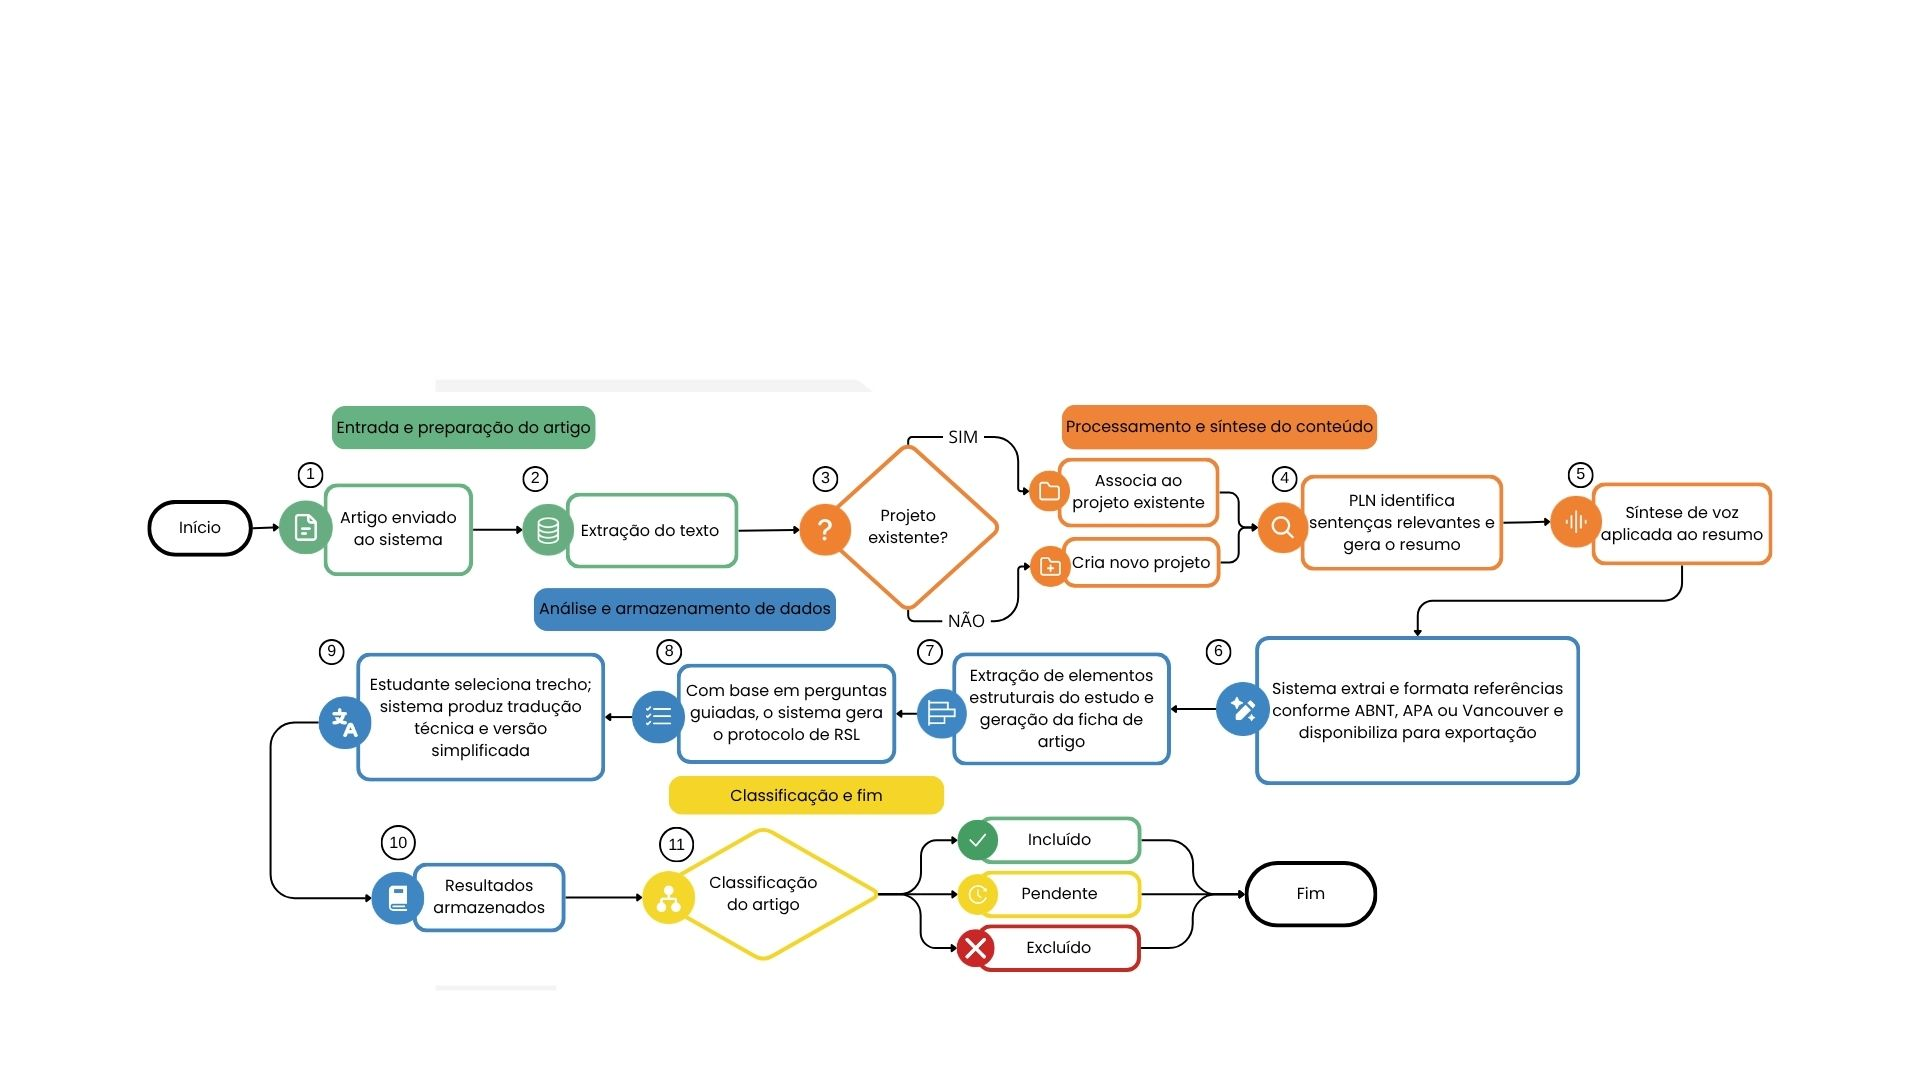
\includegraphics[width=\paperwidth,height=\paperheight]{imgs/img_006.jpg}%
}
\begin{frame}[t]{Metodologia}
  
{\scriptsize O \textbf{Aura} processa artigos em \textbf{11 etapas}: do envio do PDF até a classificação final no projeto de revisão sistemática.}

\end{frame}
}

\section{Apresentação Prática}

{
\usebackgroundtemplate{%
  
\includegraphics[width=\paperwidth,height=\paperheight]{imgs/img_007.jpg}%
}
\begin{frame}[b]{Apresentação Prática}
    \begin{itemize}
    \item \parbox{0.60\textwidth}{\textbf{Aura}: RSL inteligente na prática}
    \item \parbox{0.60\textwidth}{6 recursos \textbf{PLN} para sua revisão}
    \item \parbox{0.60\textwidth}{\textbf{Design acessível} e sem instalação}
    \item \parbox{0.60\textwidth}{\textbf{Menos tempo} de triagem, mais análise}
    \item \parbox{0.60\textwidth}{\textbf{Revisão Sistemática} simplificada}
\end{itemize}
  
  \vfill
  
  {\fontsize{4}{5}\selectfont\textit{Fonte: Autoria própria (2026)}\hfill\textcolor{black}{Imagem: Notebook com tecnologia integrada}}
\end{frame}
}

% Slide Informações Gerais (clone)
{
\usebackgroundtemplate{%
  
\includegraphics[width=\paperwidth,height=\paperheight]{imgs/img_022.jpg}%
}
\begin{frame}[b]{}
  \vspace{0.2cm}
  
  \hspace*{0.25\paperwidth}{\Large \textbf{Obrigado!}}
  
  \vfill
\end{frame}
}

\end{document}
